
\label{chap:sepsis}
\section{Sepsis and Vasomotion}

\textit{Sepsis is a condition, that develops through systemic inflammatory response syndrome (SIRS) with presence of an infection or bacteria within the body. Sepsis adversely affect heart rate, blood pressure, oxygen extraction and body temperature and leads in worst case to multi organ failure.\cite{pluta2010,kanta2014}}

Since sepsis is based on an inflammation the body activates the inflammatory cascade as an immune response. Some factors released by the inflammatory cascade have influence on vasodilation and trigger a dispersed systemic vasodilation and decrease the responsiveness of the affected vasculature. It is know that sepsis leads to imbalance of the microcirculation. The blood distribution becomes unequally. Areas with a lack of blood supply which have already a need of blood get less whereas areas with sufficient supply get more of the available amout of blood. As an adequate oxygen supply requires a sufficient circulation, the condition of the areas with a lack of blood supply deteriorates.
Local microcirculatory in several organs like kidneys or liver is impaired what leads to failure of these organs by persist of this situation.\cite{baudouin2008,kanta2014}

The vascular endothelium is an issue within the incidents of sepsis. Stressful environments like sepsis activate vascular endothelial cells. Normally it is an protective response, but in sepsis where the disorder remains, this response exaggerates unpredictable. The endothelial probity get lost and causes cell injury and hypoxia. Moreover the tissue underlying the capillaries suffer from the obstructed capillary perfusion and related hypoxia. The scheme in figure \ref{fig:Sepsis} shows the role of vascular endothelium on the way to organ failure.\cite{baudouin2008}

\begin{figure}[H]
	\centering	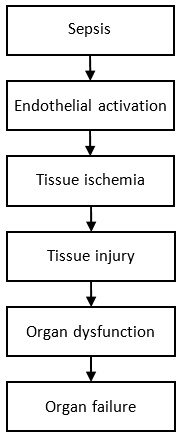
\includegraphics[width=0.2\textwidth]{figures/SepsisEndo}
	\caption{Scheme the vascular endothelium impacts during sepsis. Modified from\cite{baudouin2008}.}
	\label{fig:Sepsis}
\end{figure}

Summarized, sepsis affects the processes within the microcirculation to an extent that the impairment exceed the autoregulation abilities of vasomotion.